% !TeX root = ../../../book.tex
\section{智力谜题}\label{sec:section1.4}

让我们把迄今为止讨论过的一些原则付诸实践。具体来说,让我们研究一些有趣的数学难题并解释如何解决它们。这些问题都不涉及除基本代数和算术之外的知识,但这并不意味着它们``基础''或``简单'',因为解决并理解这些问题都涉及批判性思维技能和敏锐的洞察力。在此过程中,我们将运用我们已经提出的一些逻辑思想。我们可能需要用到多项式函数,或者用代数方法求解一些方程。我们可能需要仔细考虑论证的顺序和流程,确保一切都遵循前面的知识或推论。总的来说,我们还应该思考什么构成了我们发现事实的良好且有效的\emph{证明}!

% !TeX root = ../../../book.tex
\subsection{消失的钞票}

\subsubsection*{问题描述}

这个经典的谜题包含在一个关于分摊酒店房间费用的故事中:

\begin{quote}
    三个朋友自驾旅行,深夜入住酒店。值班店员说当晚只剩一间空房,三人合住需付 $30$ 美元。他们疲惫不堪,便同意合住,每人各付 $10$ 美元预付款。店员道谢后递过钥匙,三人随即去车上取行李。此时,前来换班的另一名店员发现前一名店员多收了房费:实际只需 $25$ 美元。于是他从收银机取出一张 $5$ 美元钞票,递给值班服务生说:``把钱退给 29 号房的客人,我们多收费了。''服务生点头后走向三人房间。客人开门时对退款又惊又喜。为公平起见,一人将钞票换成五张 $1$ 美元纸币,每人取回 $1$ 美元,剩余 $2$ 美元作为小费给了服务生。服务生道谢后离开。

    现在,三人每人实际支付 $9$ 美元房费,加上 $2$ 美元小费,总计 $29$ 美元。但他们最初支付了 $30$ 美元……消失的 $1$ 美元去哪儿了?!
\end{quote}

请仔细思考一下,然后再翻页阅读解答。

\clearpage

\subsubsection*{解答:追踪资金流向}

你搞明白了吗?其实没有任何东西凭空``消失''。这个谜题的目的就是迷惑读者,误导他们去寻找不存在的事物。题目中的数字经过精心设计,使``消失的金额''仅为 $1$ 美元,让读者误以为发生了什么神秘事件。但通过细致的逻辑分析,你会发现最终提问本身并不合理:它利用了读者对情境的误解,使其忽视逻辑推理。若数字差异变得更大,人们便不会执着于寻找``消失的钞票''。

首先,让我们分析一下在这个特殊案例中到底发生了什么。关键在于厘清资金的实际流向。我们可将参与者分为两组:朋友群体(记为 $F$)和酒店员工群体(包括店员与服务生,记为 $H$)。现在,让我们重现资金转移步骤:

\begin{enumerate}
    \item $F$ 支付 $H \quad 30$ 美元(原始房费)
    \item $H$ 退还 $F \quad \enspace 5$ 美元(多收房费退款)
    \item $F$ 支付 $H \quad \enspace 2$ 美元(服务生小费)
    \item 净变化:$F$ 向 $H$ 支付 $30 \text{\ 美元} -5 \text{\ 美元} + 2 \text{\ 美元} = 27 \text{\ 美元}$
\end{enumerate}

这样就清晰了:退款 $5$ 美元使实际房费变为 $25$ 美元,三人每人付了 $9$ 美元,再加上服务生的小费,共计 $27$ 美元。谜题错误地将小费与房费相加,但 $27$ 美元已包含全部支出。通过追踪群体间的资金流动,我们能准确还原交易过程。

\subsubsection*{泛化:改变数字}

让我们应用上述方法来修改问题,通过改变数字消除对``消失的钞票''的情感依赖,同时放大金额差异。首先定义变量表示各步骤的金额。与其``测试''特定数值,不如引入变量实现``一次性全面验证''。

设 $3n$ 表示三人首次支付的房费总额($n$ 为每人支付金额)。退款金额设为 $3r + 2$,其中 $r$ 为每人实际退款,$2$ 为给服务生的小费。下面用变量重述该问题:

\begin{quote}
    三个朋友自驾旅行,深夜入住酒店。值班店员说当晚只剩一间空房,三人合住需付 $3n$ 美元。他们疲惫不堪,便同意合住,每人各付 $n$ 美元预付款。店员道谢后递过钥匙,三人随即去车上取行李。此时,前来换班的另一名店员发现前一名店员多收了房费:实际只需 $3n - (3r + 2)$ 美元。于是他从收银机取出一张 $3r + 2$ 美元钞票,递给值班服务生说:``把钱退给 29 号房的客人,我们多收费了。''服务生点头后走向三人房间。客人开门时对退款又惊又喜。为公平起见,三人每人取回 $r$ 美元,剩余 $2$ 美元作为小费给了服务生。服务生道谢后离开。

    现在,三人每人实际支付 $n-r$ 美元房费,加上 $2$ 美元小费,总计 $3(n-r)+2$ 美元。但他们最初支付了 $3n$ 美元……消失的 $3n - [3(n - r) + 2]=3r - 2$ 美元去哪儿了?!
\end{quote}

现在问题是否更清晰了?正如我们之前解释的那样,差异源于原文将小费加入退款后的房费,再与初始 $3n$ 美元房费进行比较。正确的比较应该是,实际房费支出 $3(n-r) = 3n - 3r$,与退费后房费与小费之和 $[3n-(3r+2)] + 2 = 3n-3r$ 进行比较。两者完全相等!

\subsubsection*{泛化:留给你的问题}

谜题的原始陈述中,$n=10, r=1$,因此``消失的钞票''神奇地变为 $3r-2=1$。如果我们选择更大的数值——例如 $n=100, r=10$——那么 $300$ 美元的房间实际花费 $268$ 美元,服务生会退还三人 $32$ 美元,他们每人拿回 $10$ 美元,服务生保留 $2$ 美元,差额就变成了 $28$ 美元。真的会有人相信 $28$ 美元在此交易中凭空消失了吗?如果我们使用更大的 $n$ 和 $r$ 值呢?你能把差额扩大到多大?或缩小到多小?给定所需的差额(以美元为单位),你能找到满足条件的 $n$ 和 $r$ 的值吗?有多少种方法可以做到这一点?

\subsubsection*{解题心得}

逻辑和理性思维在解决难题时至关重要,因为情绪容易误导人。如果我们最初将这个谜题表述为``消失的 $28$ 美元'',你会有同样的反应吗?在试图回溯并弄清真相之前,你是否会感到短暂的困惑?


% !TeX root = ../../../book.tex
\subsection{高斯驾到}\label{sec:section1.4.2}

\subsubsection*{问题描述}

数学界流传着一个关于史上最伟大数学家兼物理学家之一——卡尔·弗里德里希·高斯 (Carl Friedrich Gauss) 的著名轶事。无论故事真实与否,其魅力令无数人深信不疑。高斯活跃于 18 世纪末至 19 世纪中叶,在数论、复分析、光学、几何学及天文学等诸多领域做出了奠基性贡献。请阅读下面这则故事,设想自己(无论童年或现在)会如何应对,然后再继续探讨。

\begin{quote}
    清晨,小学教室里喧闹的学生令老师不胜其烦。为获得片刻安宁,他急需让学生们专注做事。老师高声要求学生取出石板和粉笔。待众人准备就绪,他布置了一道题目:计算从 $1$ 到 $100$ 所有整数之和,并承诺最先完成者可担任当日助教。老师回到座位,料想繁重的计算将让学生们安静许久。不料仅过一分钟,一个男孩便带着写有答案的石板前来。老师惊讶之余亲自验算,结果证实男孩答案完全正确。他是如何快速完成计算的?
\end{quote}

请认真思考后再翻阅解答。请注意:这则故事``发生''在计算器尚未问世的年代,解题只能依靠纸笔与心算能力。

\clearpage

\subsubsection*{解答:简化计算}

也许你已经找到了窍门。实际上,这个问题有多种解法,它们大多基于相同的核心思路:尽量减少所需的计算量。

如果简单地遍历这 $100$ 个数字并逐个累加,需要进行 $99$ 次加法,且运算数字会越来越大。当然,技巧不仅仅在于更快地执行加法,而在于从根本上提高计算效率。我们知道,乘法本质上是数字与其自身的重复加法。因此,如果能找到合适的数字进行重复自加,就有可能将大量加法简化为一次乘法。

另一个关键点是加法满足\textbf{结合律}和\textbf{交换律},这意味着加法的顺序不影响最终结果。具体而言,无论将数字从 $1$ 加到 $100$ 还是从 $100$ 加到 $1$,其总和 $S$ 都相同。我们可以这样表示:
\begin{center}
    \begin{tabular}{ccccccccccccccc}
          1 & + &   2 & + &   3 & + & \dots & + &  98 & + &  99 & + & 100 & = & S\\\noalign{\smallskip\smallskip}
        100 & + &  99 & + &  97 & + & \dots & + &   3 & + &   2 & + &   1 & = & S\\\noalign{\smallskip\smallskip}
        \hline
        101 & + & 101 & + & 101 & + & \dots & + & 101 & + & 101 & + & 101 & = & 2S\\\noalign{\smallskip\smallskip}
    \end{tabular}
\end{center}
注意,我们以两种顺序写出了总和 $S$。将这两个等式逐项相加,得到总和 $2S$ 的表达式。这个新表达式可直接转换为乘法,因为有 $100$ 项,每项都等于 $101$。因此:
\begin{align*}
    2S &= 101 \cdot 100 \\
     S &= 101 \cdot 50 = 5050
\end{align*}
这比执行 $99$ 次加法要快得多。事实上,只要稍加练习,我们完全能在脑海中完成整个计算过程!

\subsubsection*{另一种解法:配对法}

解决该问题的相似思路是省去两行相加的中间步骤,直接将原始求和中的数字配对,如下所示:
\begin{align*}
    S &= 1 + 2 + 3 + \dots + 98 + 99 + 100 \\
    &= (1 + 100) + (2 + 99) + (3 + 98) + \dots + (49 + 52) + (50 + 51) \\
    &= 101 + 101 + \dots + 101 = 50 \cdot 101 = 5050
\end{align*}
该方法与前述解法本质相同,均利用加法交换律和结合律重组求和项,只是跳过了求 $2S$ 表达式然后再除以 $2$ 这一中间步骤。

\subsubsection*{泛化:$n$ 为偶数}

如果老师要求学生计算 $1$ 到 $1000$ 的数字之和呢?学生是否会抗议?高斯能否同样迅速作答?我们虽不确定前两个问题的答案,但相信你一定能轻松解决。这里唯一不同的是,我们需要创建 $500$ 组配对(而非 $50$ 组),每组之和为 $1001$(而非 $101$),因此结果为
\[1 + 2 + 3 + \dots + 998 + 999 + 1000 = 1001 \cdot 500 = 500500\]

看起来是不是存在某种规律呢?你觉得你能在不进行乘法的情况下立即说出 $1$ 到 $100$ 万之间所有数字之和是多少吗?

\subsubsection*{泛化:$n$ 为奇数}

如果老师要求的是前 $99$ 个数字之和呢?配对法是否仍然适用?让我们验证一下:
\begin{align*}
    S &= 1 + 2 + 3 + \dots + 97 + 98 + 99 \\
    &= (1 + 99) + (2 + 98) + (3 + 97) + \dots + (48 + 52) + (49 + 51) + 50 \\
    &= (49 \cdot 100) + 50 = 4950
\end{align*}
请注意,总项数为奇数,因此无法将所有数字完全配对,必须在乘法结果上加上中间项 $50$。是否有其他配对方式?
\begin{align*}
    S &= 1 + 2 + 3 + \dots + 97 + 98 + 99 \\
    &= (1 + 98) + (2 + 97) + (3 + 96) + \dots + (48 + 51) + (49 + 50) + 99 \\
    &= (49 \cdot 99) + 99 = 50 \cdot 99 = 4950
\end{align*}
这种方法\emph{看起来}与原始谜题的结果更相似,因为我们只执行\emph{一次}乘法。这是巧合吗?请尝试用相同方法计算其他奇数项之和:前 $7$ 个整数之和是多少?前 $29$ 个呢?前 $999$ 个呢?前 $999999$ 个呢?

\subsubsection*{泛化:任意 $n$}

让我们从个案研究中抽离出来,尝试从更一般的视角解决这个问题。假设老师向学生提出了以下问题:
\begin{quote}
    给出前 $n$ 个自然数之和的公式。我需要一个具体的公式,这样当有人告诉我 $n$ 的值时,我就能直接代入并快速得到答案。
\end{quote}

第二句的说明排除了其他方法。虽然我们之前提出过一些简单算法,但现在被要求给出一个直接计算的公式。该如何入手呢?根据之前的观察,分情况讨论 $n$ 的奇偶性是一个合理的策略。我们发现奇偶情况下的配对结果略有差异,因此先讨论其中一种情况,再讨论另一种。在每种情况下,我们都寻求 $S(n) = 1 + 2 + 3 + \dots + (n - 2) + (n - 1) + n$ 的表达式。这里用 $S(n)$ 表示这个和依赖于 $n$ 的值。

如果 $n$ 为偶数,我们可以将所有数完美配对:
\begin{align*}
    S(n) &= 1 + 2 + 3 + \dots + \left(\frac{n}{2}-1\right) + \frac{n}{2} + \left(\frac{n}{2}+1\right) + \dots + (n - 2) + (n - 1) + n\\
    &=  (1 + n) + \left(2 + (n - 1)\right) + \left(3 + (n - 2)\right) + \dots + \left(\left(\frac{n}{2}-1\right)+\left(\frac{n}{2}+2\right)\right) + \left(\frac{n}{2}+\left(\frac{n}{2}+1\right)\right) \\
    &= (n+1)\frac{n}{2} = \frac{n^2+n}{2}
\end{align*}

将已知结果的偶数(如 $n=100, 1000, 1000000$)代入公式进行验证。注意,公式中出现 $\frac{n}{2}$ 是合理的,因为 $n$ 为偶数,$\frac{n}{2}$ 必为整数。

如果 $n$ 为奇数呢?此时无法将所有数完全配对,需要巧妙处理。回想前 $99$ 项求和的方法,通过暂时忽略末项 $n$,将剩余项配对。有趣的是,每对之和恰好等于末项 $n$。让我们尝试运用此方法:
\begin{align*}
    S(n) &= 1 + 2 + 3 + \dots + \left(\frac{n-1}{2}-1\right) + \frac{n-1}{2} + \left(\frac{n-1}{2}+1\right) + \dots + (n - 2) + (n - 1) + n\\
    &=  \left(1 + (n-1)\right) + \left(2 + (n - 2)\right) + \dots + \left(\left(\frac{n-1}{2}\right)+\left(\frac{n-1}{2}+1\right)\right) + n \\
    &= n+n+ \dots + \left(\frac{2n-2}{2}+1\right) +n = (n+n+\dots+n)+n
\end{align*}

这表明每对数字之和为 $n$,即我们最初忽略的末项。现在计算配对数量:第一对是 $(1, n - 1)$,第二对是 $(2, n - 2)$,依此类推,最后一对的首项为 $\frac{n-1}{2}$。因此共有 $\frac{n-1}{2}$ 对。(注意 $n$ 为奇数保证了 $n-1$ 为偶数,故 $\frac{n-1}{2}$ 为整数。请回顾推导过程,确认每一步的有效性。)加上末项 $n$,总和可表示为:
\[S(n) = \left(\frac{n-1}{2} + 1\right) \cdot n = \left(\frac{n-1}{2} + \frac{2}{2}\right) \cdot n = \frac{n+1}{2} \cdot n = \frac{n^2+n}{2}\] 

令人惊讶的是,这与 $n$ 为偶数时得到的公式完全相同!你是否感到意外?虽然奇偶情况的解法相似,但并无明显迹象预示结果会一致。这对我们有什么启示?数学家面对这种``巧合''时,会思考是否存在\emph{更简洁}、\emph{更普适}的解法——能否用一种方法同时处理奇数和偶数\emph{两种}情况?既然结果相同,这样的方法很可能存在。请在继续阅读前先思考一下这个问题。

\subsubsection*{泛化:任意 $n$, \emph{不}分开讨论}

事实证明,我们在之前讨论这道谜题时已经暗示过另一种方法。还记得将正序求和写在一行、倒序求和写在另一行并将它们相加吗?当时处理奇偶性问题时,我们因看似步骤繁琐而避开了此法;``配对法''似乎更快捷,所以我们便采用了配对法。但若重新审视``两次相加''这一方法,会得到什么?我们会发现:
\begin{center}
    \begin{tabular}{ccccccccccc}
           1  & + &     2 & + & \dots & + & (n-1) & + &     n & = & S(n)\\\noalign{\smallskip\smallskip}
           n  & + & (n-1) & + & \dots & + &     2 & + &     1 & = & S(n)\\\noalign{\smallskip\smallskip}
        \hline
        (n+1) & + & (n+1) & + & \dots & + & (n+1) & + & (n+1) & = & 2S(n)\\\noalign{\smallskip\smallskip}
    \end{tabular}
\end{center}
此时第三行求和包含 $n$ 项,每项均为 $(n + 1)$。因此:
\begin{align*}
    2S &= (n+1) \cdot n \\
     S &= \frac{1}{2}(n+1) \cdot n = \frac{n^2+n}{2}
\end{align*}
这正是此前推导的公式,而此处的推导过程完全不依赖 $n$ 的奇偶性!(请回顾上述步骤并自行验证 $n$ 的奇偶性确实无关紧要。)

\subsubsection*{第三种解法:可视化图表}

在结束此问题之前,我们介绍一种几何解法。我们将求和 $S(n)$ 与正方形的面积关联,并将求和的各项($1, 2, 3, \dots, n - 1, n$)可视化为正方形的一部分。具体来说,考虑一个 $n \times n$ 的正方形,并将各项表示为宽度为一个单位、高度递增的矩形。见下图:

\begin{center}
    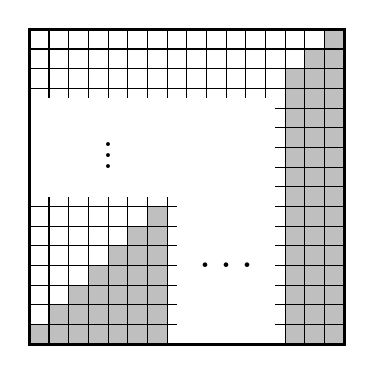
\begin{tikzpicture}[scale=0.5, x=0.5cm, y=0.5cm, font=\LARGE]
        \foreach \x in {0,...,15} 
            \foreach \y in {0,...,15}
                {
                    \pgfmathparse{(\x >= \y && (\x<7 || \x>12)) ? "lightgray" : "white"}
                    \edef\colour{\pgfmathresult}
                    \path[fill=\colour] (\x,\y) rectangle ++ (1,1);
                    \draw[black] (\x,\y) rectangle ++ (1,1);
                }
        \fill[white] (0, 7.5) rectangle ++ (8,5) node[color=black, pos=.5, align=center]{$\vdots$};
        \fill[white] (7.5, 0) rectangle ++ (5,8) node[color=black, pos=.5, align=center]{$\dots$};
        \fill[white] (7.5, 7.5) rectangle ++ (5,5) node[color=black, pos=.5, align=center]{$\iddots$};
        \draw[very thick, black] (0, 0) rectangle ++ (16,16);
    \end{tikzpicture}
\end{center}

现在,要求 $S(n)$ 的公式等价于计算正方形内所有矩形覆盖的\emph{面积}。直接相加各矩形面积只是重复原问题,因此我们需要将该面积与正方形的总面积关联。为此,考虑剩余区域,如何描述未被矩形覆盖的部分?观察第一个 $1 \times 1$ 矩形正上方的区域:它是一个尺寸为 $(n - 1) \times 1$ 的矩形。

类似地,$2 \times 1$ 矩形上方的区域是一个 $(n-2) \times 1$ 矩形。此模式持续下去!最终,在 $(n - 1) \times 1$ 矩形上方为一个 $1 \times 1$ 矩形,而最后一个 $n \times 1$ 矩形上方无区域。这些矩形的总面积类似于 $S(n)$,但缺少最后一项 $n$。现在,将所有矩形的面积与 $S(n)$ 和正方形面积关联:
\[n^2 = S(n) + (S(n) - n) = 2S(n) - n\]
解得
\[S(n) = \frac{n^2+n}{2}\]
与我们之前得到的公式一致!

\subsubsection*{解题心得}

有时,问题有多种解法。有些方法易于构思但难于求解;有些难以想到但求解简洁;还有些可能根本无效!通常无法预判哪种方法有效,因此建议动手尝试并观察结果。记录尝试的过程和结果,以便后续重新评估。这是数学学习中需牢记的原则:我们并非总能立即知晓正确路径,偶尔会陷入困境或走入死胡同。这不应令人沮丧;它是学习的一部分。

作为练习,尝试为 $n$ 为奇数的情况重新``配对'',不忽略求和的最后一项,而是分离中间项并将数字从外向内配对。这会得到相同结果吗?该方法是否比原解法更简便、更快速或有所不同呢?或者,对于 $n$ 为偶数的情况,令 $n=2k$ 会怎样?对于 $n$ 为奇数又该如何操作?这种表示会改变处理过程吗?会使问题更容易处理吗?现在,你能构思一种全新的解法吗?


% !TeX root = ../../../book.tex
\subsection{求和杂谈}\label{sec:section1.4.3}

\subsubsection*{奇数求和:观察模式}

既然谈到了整数求和,那就让我们来看一些相关的问题。首先,我们将介绍一种解释奇数之和的有趣得几何方法:让我们将 $1$ 表示为 $1 \times 1$ 块,然后将每个连续增大的奇数表示为角为 $1 \times 1$ 块的直角,完美贴合前一个这样的图。我们为什么要这样做?因为都是奇数,连续项的大小相差为 $2$,每次将角块的边延长 $1$,可以让直角与原图形紧密地相互贴合并逐渐构建起更大的正方形!

\begin{center}
    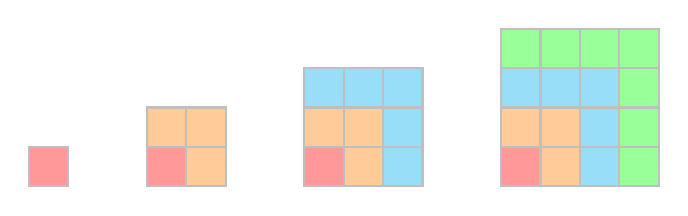
\begin{tikzpicture}[thick,scale=0.5, x=1cm, y=1cm]
        \foreach \x in {0,3,7,12}
        {
            \fill[red!40!white] (\x, 0) rectangle ++ (1,1);
            \draw[lightgray] (\x, 0) rectangle ++ (1,1);
        }

        \foreach \x in {3,7,12}
        {
            \foreach \i in {0,1}
            {
                \fill[orange!40!white] (\x+\i, 1) rectangle ++ (1,1);
                \draw[lightgray] (\x+\i, 1) rectangle ++ (1,1);
                \fill[orange!40!white] (\x+1, \i) rectangle ++ (1,1);
                \draw[lightgray] (\x+1, \i) rectangle ++ (1,1);
            }
        }

        \foreach \x in {7,12}
        {
            \foreach \i in {0,...,2}
            {
                \fill[cyan!40!white] (\x+\i, 2) rectangle ++ (1,1);
                \draw[lightgray] (\x+\i, 2) rectangle ++ (1,1);
                \fill[cyan!40!white] (\x+2, \i) rectangle ++ (1,1);
                \draw[lightgray] (\x+2, \i) rectangle ++ (1,1);
            }
        }

        \foreach \i in {0,...,3}
        {
            \fill[green!40!white] (12+\i, 3) rectangle ++ (1,1);
            \draw[lightgray] (12+\i, 3) rectangle ++ (1,1);
            \fill[green!40!white] (12+3, \i) rectangle ++ (1,1);
            \draw[lightgray] (12+3, \i) rectangle ++ (1,1);
        }
    \end{tikzpicture}
\end{center}

这种模式会持续下去吗?如果我们相信确实如此,我们如何证明这一点呢?这种几何图案的数值之和意味着什么?这是一个首先要回答的好问题,因为尽管几何图案很漂亮,但却很难使用和操作,最终也难以给出明确地\emph{证明}。本质上,对着模式的前几项说:``看,它有效!'' 并不构成官方的数学证明,因此我们必须找到更好的方法来表述这个问题。这并不是要淡化我们注意到的图案的意义和美丽;有趣的是,它的工作方式确实为我们提供了一些有价值的见解,让我们从数学上了解可能发生的事情,但归根结底,这就是它能为我们做的一切。

\subsubsection*{奇数求和:证明我们的发现}

让我们尝试用数字形式写出上图所表示的求和。 角块由 $1 \times 1$ 块组成,每个角比前一个多两块,因此我们看到的每个正方形都可以由一个和表示,例如
\[1 \:\text{ 或 }\: 1+3 \:\text{ 或 }\: 1+3+5 \:\text{ 或 }\: 1+3+5+7 \]
以此类推。我们从这些项中注意到,它们其实是平方数
\[1=1^2 \quad 1+3=4=2^2 \quad 1+3+5=9=3^2 \quad 1+3+5+7=16=4^2 \]
\emph{这}才是我们想要证明的模式;它相当于我们之前注意到的几何图案,但现在它是用我们可以操作的术语编写的。现在让我们思考一下如何才能做到这一点。这种模式与我们之前见过的模式相似吗?我们已经证明了关于整数和的结果了吗?当然!回顾之前的题目;(事实上,在某些方面)我们证明了
\[1 + 2 + 3 + \dots + (n_1) + n =\frac{n^2 + n}{2}\]
这对于该题有何用处?我们证明的求和公式涉及从 $1$ 到 $n$ 的\emph{所有}连续整数,但对于当前要求的公式,我们只想考虑连续\emph{奇数}。

之前我们用函数 $S(n)$ 表示前 $n$ 个自然数之和,所以我们定义函数 $T(n)$ 表示前 $n$ 个奇数之和。现在,我们首先需要确定该和的项,然后以某种方式将它们与 $S(n)$ 联系起来。下面,我们写出了 $n = 1,2,3 ,4$ 时的和。你能找到一种方法来识别求和中的最大项并用 $n$ 表示它吗?
\begin{align*}
    n=1: &\quad 1\\
    n=2: &\quad 1+3\\
    n=3: &\quad 1+3+5\\
    n=4: &\quad 1+3+5+7\\
\end{align*}
请注意,求和项的最后一项始终为 $2n-1$。这与一个普遍事实有关,即对于某个特定整数 $k$,任何偶数整数都可以表示为 $2k$,对于某个特定整数 $n$,任何奇数整数都可以表示为 $2n - 1$。(对于某个整数,我们也可以将奇数表示为 $2n + 1$,不过,这里使用 $2n - 1$ 更方便。)因此,我们要求的前 $n$ 个奇数之和的公式为
\[T(n) = 1 + 3 + 5 + 7 + \dots + (2n - 3) + (2n - 1)\]
我们可以将这个求和公式与 $S(n)$ 或类似的公式联系起来吗?请注意求和公式
\[S(2n) = 1 + 2 + 3 + \dots + (2n - 3) + (2n - 2) + (2n - 1) + 2n\]
包含从 $1$ 到 $2n$ 的\emph{所有}自然数,而 $T(n)$ 仅包含该范围内的奇数。也许两个和相减并尝试找到剩余项之和的表达式是有意义的:
\begin{align*}
    S(2n) - T(n) &= 1 + 2 + 3 + \dots + (2n - 1) + 2n \\
    &\quad -\big(1 + 3 + 5 + \dots + (2n - 3) + (2n - 1)\big) \\
    & =  2 + 4 + 6 + \dots + (2n - 2) + 2n
\end{align*}
这些项都是从 $2$ 到 $2n$ 的\emph{偶数}。我们怎样才能得到这个求和公式呢?我们是否需要做额外的工作,还是可以应用之前的证明结果?由于所有项都是\emph{偶数},我们可以将所有项除以 $2$ 并写成
\begin{align*}
    \frac{1}{2}\big(S(2n) - T(n)\big) &= \frac{1}{2}\big(2 + 4 + 6 + \dots + (2n - 2) + 2n\big)\\
    &= 1 + 2 + 3 + \dots + (n - 1) + n = S(n)
\end{align*}
我们可以保证,最右边的求和公式中的所有项都是整数。不仅如此,它们\emph{都是}从 $1$ 到 $n$ 的连续整数,并且我们知道它们的求和公式!现在,\text{一切都是用我们已知的公式}(即 $S(n)$ 和 $S(2n)$)以及我们要求的公式(即 $T(n)$)书写的。最后一步要做的是整理方程,分离 $T(n)$,然后代入我们已知的 $S$ 的公式:
\begin{align*}
    \frac{1}{2}\big(S(2n) - T(n)\big) &= S(n) \\
    S(2n) - T(n) &= 2S(n) \\
    T(n) &= S(2n) - 2S(n) \\
    T(n) &= \frac{(2n)^2 + 2n}{2} - \frac{2 \cdot (n^2 + n)}{2} \\
    T(n) &= \frac{4n^2 + 2n - 2n^2 - 2n}{2} \\
    T(n) &= \frac{2n^2}{2} \\ 
    T(n) &= n^2
\end{align*}
这看起来相当不错,不是吗?尽管必须完成一些代数步骤,我们还是得出了我们希望证明的结论:连续奇数的和是完全平方数。不仅如此,我们还成功地精确证明了该平方数与求和项数之间的关系。 具体来说,我们刚刚证明的结论的一种简洁概括描述是``前 $n$ 个奇数之和等于 $n^2$''。

\subsubsection*{另一种解法:归纳证明}

我们可以用不同的方式证明这一点吗?如果我们还没有证明上一节的结论,或者我们没有想到以这种方式证明它怎么办?我们能否以某种方式利用我们最初注意到的和的几何结构?

让我们回过头来用稍微不同的方式思考这个问题。具体来说,让我们看看为什么在求和中再添加一项会产生另一个平方数。假设我们已知其中一个求和产生一个平方数;我们知道这对于第一个求和 ($1 = 1^2$) 是正确的,但我们假设对于任意数量的项 $n$ 都会发生这种情况。也就是说,对于某个值 $n$, 我们\emph{假设}
\[1 + 3 + 5 + \dots + (2n - 3) + (2n - 1) = n^2\]
基于这一事实,我们接下来可以推断出下一个和是什么吗?当我们向求和中再添加一项时,我们会加上下一个奇数 $2n + 1$,所以让我们看看这会如何影响求和结果:
\[1 + 3 + 5 + \dots + (2n - 3) + (2n - 1) + (2n + 1) = n^2 + 2n + 1 = (n + 1)^2\]
这似乎证实了我们的想法,不是吗?知道求和的表现方式与我们预期的一致(``如果前 $n$ 个奇数整数之和为 $n^2$……'')我们就可以推断下一个和也必须以相同的方式表出现(……那么前 $n+1$ 个奇数整数的和是 $(n+1)^2$'')。这也证明了结论吗?你觉得怎么样?本质上假设我们的结论成立来进一步证明它,这感觉很奇怪吗?我们真的是这么做的吗?

这种证明策略 --- 使用结果的一种形式来证明结果的``后续''形式 --- 称为\textbf{数学归纳法}。(一般来说,``后续''一词的含义取决于上下文;在这里,它的意思是再加上一项后和。)我们将在下一章更详细地研究这一策略。目前,我们先指出这是一个完美的策略,但它高度依赖于第一个求和的正确表示:$1 = 1^2$。这样,我们所做的工作使我们能够推断出第二个求和是 $(1+3=2^2)$,接着就可以推断出第三个求和是 $(1+3+5=3^2)$,以此类推……如果我们只能证明第二部分,但第一部分的结果没有按照我们想要的方式计算怎么办?我们还能证明结论吗?一般来说,这对归纳策略有何启示?稍后我们将更普遍地解决其中一些问题。

\subsubsection*{泛化:算术级数}

我们要谈的最终求和问题与我们迄今为止看到的两个问题密切相关,事实上,如果我们能证明下一个结论,就不必证明前两个结论了!从这个意义上说,下一个结论比前两个结论更强:这个结论的真实性意味着前两个结论的真实性。(这是数学术语中的常见概念,将结论标记为比其他结论更强或更弱。)

对于这个结论,我们想要发展一个通用\textbf{算术级数}。这句话的意思是我们要添加一个算术级数,其中连续项之间的差是一个固定值。另一种思考方式是,每一项都是通过前一项加上一个固定常数而来。请注意,我们在后两个题目中求和的就是算术级数:第一个求和中,每项相差 $1$(或者,每项上加 $1$ 得到下一项),第二个求和中每个项相差 $2$(或者,每项上加 $2$ 得到下一项)。

我们如何表示一个通用的算术级数?因为连续项必须相差一个固定常数,让我们为该值分配一个变量,例如 $c$,作为常数。求和中也必须有第一项,所以让我们将该值分配给一个变量,例如 $a$,因为它是第一个字母。我们还需另一个变量来告诉我们求和中有多少项,因此我们将使用 $k$ 表示项数,因为我们之前已经使用过该变量表示相同的含义。现在,我们可以用这三个变量来表示整个求和:
\[A(a, c, k) = a + (a + c) + (a + 2c) + (a + 3c) + \dots + (a + (k - 2)c) + (a + (k - 1)c)\]
我们可以利用每对连续项相差 $c$ 这一事实,使用第一项 $a$ 来表示第二项,并且我们可以通过不断增加 $c$ 来表示第三项,依此类推。我们总共需要 $k$ 项,因此,将第一项视为 $a+ 0 \cdot k$,最后一项是我们将 $c$ 添加到第一项 $k - 1$ 次后得到的结果(从 $0$ 到 $k - 1$(含) 有 $k$ 个数字)。另请注意,我们引入了符号 $A(a, c, k)$ 来表示``第一项 $a$、常数差 $c$ 和 $k$ 项的算术级数之和''。现在,我们怎样才能算出这个和呢?

让我们采用以前有效的策略:在第一个求和题目中,我们正序和倒序写下求和项并将它们加在一起。这会创建许多具有相同求和结果的项对,从而将求和简化为乘法。如果我们在这里这样做时会发生什么?我们看到

\begin{center}
    \begin{tabular}{ccccccccc}
                 a & + &      (a+c) & + & \dots & + & (a+(k-1)c) & = & A(a,c,k)\\\noalign{\smallskip\smallskip}
        (a+(k-1)c) & + & (a+(k-2)c) & + & \dots & + &          a & = & A(a,c,k)\\\noalign{\smallskip\smallskip}
        \hline
        (2a+(k-1)c)& + & (2a+(k-1)c)& + & \dots & + &(2a+(k-1)c) & = &2A(a,c,k)\\\noalign{\smallskip\smallskip}
    \end{tabular}
\end{center}
我们再次发现配对项都有相同的和,在这种情况下,和是 $2a+ (k-1)c$。这样的配对项有多少对?正好是 $k$ 个项!(这就是我们选择使用该变量的原因。)将求和表示为乘法,我们现在可以推出
\[2A(a, c, k) = k \cdot (2a + (k - 1)c)\]
因此
\[A(a, c, k) = \frac{k}{2} \cdot k \cdot (2a + (k - 1)c)\]
这看起来符合你的期望结果吗?你的预期是什么?有时,尝试``猜测''可能会发生什么,然后看看结果是否与你的直觉相符,以及如何相符,会有所帮助。

\subsubsection*{具体应用}

上面提到过,我们之前题目中的求和都是算术级数,那么这个公式是否可以得出这些求和的正确结果呢?在第一题中,变量值为 $a = 1,c = 1, k = n$;代入这些值会得到
\[A(1, 1, n) = \frac{1}{2} \cdot k \cdot (2 + (n - 1)) = \frac{n}{2} \cdot(n+1) = \frac{n^2+n}{2}\]
这确实是我们之前得到的结论。那第二题呢?变量的值是多少?公式正确吗?这些问题请你来验证结果。

\subsubsection*{另一种表示}

这个问题的最后,我们想讨论另一种表示刚刚推导出的公式的方法。查看括号中的项,并以稍微不同的方式书写:$a+ (a+ (k-1)c)$。这些项看起来特别有趣吗?是的,它们分别是求和的第一项和最后一项。这为我们提供了一种不同的方式来表达我们推导出的求和公式:$A(a, c, k) = \frac{k}{2}(a + b)$,其中 $a$ 是求和的第一项,$b$ 是最后一项。这个版本的公式可以更方便,更快捷地进行一些求和。

例如,假如我们让你求一个算术级数之和,其中第一项为 $12$,最后一项为 $110$,总共有 $14$ 项,你就不必费心费力去计算常数差 $c$;相反,你可以简单地完成求和:$\frac{14}{2} \cdot (12 + 110) = 854$。是不是快得多?该算术级数的 $c$ 值是多少?给定 $a,b,k$,有没有一种简单的方法可以快速求出 $c$?

\subsubsection*{解题心得}

了解以前的结论会很有帮助,因为它们可以使证明更简短、更容易。有时,很难知道某个特定结果何时有用,或者即使意识到它的用途,也可能很难弄清楚如何应用它。在这种情况下,我们意识到到我们之前已经证明了一个求和公式,因此至少尝试弄清楚它在证明不同的求和公式时如何发挥作用是有意义的。然而,有一种完全不同的方法可以证明奇数之和的公式,不依赖于我们之前的结论。这暗示了一个更通用的结论,好奇的数学家会尝试更通用地探索这个问题,我们通过研究任意算术级数做到了这一点。但最终,我们对前两个求和公式使用了多种策略,并且仅将其中一种策略应用于一般级数问题。我们可以在其他设定下使用这些策略吗?我们是否也可以通过归纳法来证明第一个求和公式?我们可以使用正序/逆序技术来证明第二个求和公式吗?尝试使用这些策略,看看会发生什么。这对你来说可能会很奇怪或没有必要,因为我们已经有了结论,但是了解不同技术在不同环境中如何发挥作用是一个宝贵的经验。在数学中,弄清楚在证明中使用哪种策略通常与找出证明结果一样困难(甚至更难)。考虑到这一点,练习特定的策略来培养一种直觉,知道它们何时有效以及何时需要尝试其他方法,是很有帮助的。


% !TeX root = ../../../book.tex
\subsection{好友倾向}\label{sec:section1.4.4}

\subsubsection*{问题描述}

这个问题基于以下一则关于匈牙利社会学家的轶事以及他对儿童朋友圈的观察。

\begin{quote}
    ``20 世纪 50 年代,匈牙利社会学家 S. Szalai 研究了儿童之间的友谊关系。他观察到,在任何大约 $20$ 个孩子的群体中,都能找到四个孩子是共同的朋友,或者四个孩子中没有两个孩子是朋友。在得出社会学结论之前, S. Szalai 咨询了当时三位著名的匈牙利数学家: Erdos, Turan 和 Sos 。简短的讨论后表明,这其实是一种数学现象,而非社会学现象。对于至少 $18$ 个元素上的任意对称关系 $R$,存在 $4$ 个元素的子集 $S$,使得 $R$ 包含 $S$ 中的所有对或不包含其中任何对。这一事实是 1930 年证明的拉姆齐定理(Ramsey's theorem)的一个特例,拉姆齐理论的基础,后来发展成为组合数学的一个丰富领域。 --- (引自麻省理工学院 Jacob Fox 教授的\href{https://www.a.com}{讲义}。)''
\end{quote}

现在我们遵循相同的思路提出类似的问题,但数字较小。具体来说,我们想要找出\emph{满足}其中三人相互都是朋友或敌人的最小群体规模。

\begin{quote}
    假设在一群人中,其中任意两人要么是朋友,要么是敌人,并且这是唯一可能的关系(即没有熟人或亦敌亦友或类似的关系)。以四人为一组,试着为每对指定朋友/敌人关系,使得不会有三人一组都是朋友或敌人。五个人可以实现吗?六个呢?七个?十个?二十个呢?尝试确定最小群体规模,使得你就可以\emph{保证}找到一个由三个人组成的小组,他们要么都是朋友,要么都是敌人。
\end{quote} 

请仔细思考一下,然后再翻页阅读解答。

\clearpage

\subsubsection*{有效地表述问题}

你做出来了吗?这是一个非常棘手的问题,所以如果你没有解出来,请不要感到难过。事实上,我们认为调查这个问题与实际找到答案一样重要,因为有多种方法可以解决这个问题,而且看不同的人如何解释这个问题总是很有趣。

首先,让我们讨论一下如何写下/画出/谈论这种情况。对于该题提出的任何问题,我们都应该考虑一组具有一定规模的人,并思考这群人中任意两人之间的关系。为了解决这个问题,我们需要一种高效且易于解释的方法表示所有这些关系,以便我们可以验证大小为 $3$ 的子群所需的属性。具体来说,我们想要轻松识别是否存在大小为 $3$ 的\emph{同质}子群,即三个人\emph{互为}朋友或\emph{互为}敌人。从现在起,我们将其称为``\textbf{同质性}''。

我们怎么才能做到这一点呢?我们如何才能表示人及其关系呢?我们可以对小组中的人员进行编号,然后写出所有数字对的列表,并用 $F$(朋友)或 $E$(敌人)标记每对数字的关系。让我们尝试为四人小组执行此操作:

\[12F \quad 13E \quad 14F \quad 23F \quad 24E \quad 34F\]

这群朋友/敌人满足同质性吗?验证起来并不那么容易,不是吗?首先,编号使得很难找到大小为 $3$ 的子群,为了验证属性,我们需要检查所有此类子群以确保它们不是 $E E E$ 或 $F F F$。也许在尝试解决问题之前,我们应该找到一种更好的方式来表示信息。对于群体中的所有可能配对,你能想出一种视觉上令人更加愉悦的方式来表示两个人是朋友还是敌人吗?具体来说,我们希望得到一种相对有效的方法来寻找大小为 $3$ 的子群并识别它们是否全是朋友还是全是敌人。

让我们尝试将组中的每个人表示为一个点,并根据这两个人是朋友还是敌人用一种线连接两个人。例如,我们用蓝线表示朋友,用红线表示敌人(记住,任何两个人要么是朋友,要么是敌人,没有别的可能,所以每对点必然有彩色线连接它们)。例如,下图描述了我们在上面分配的关系和符号:

\begin{center}
    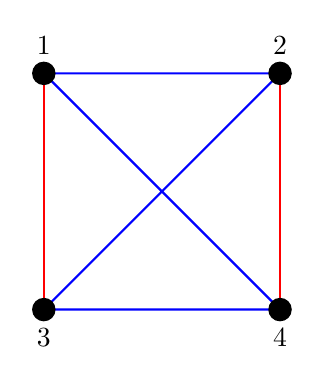
\begin{tikzpicture}[thick,scale=0.5]
        \coordinate (A) at (0,6);
        \coordinate (B) at (6,6);
        \coordinate (C) at (0,0);
        \coordinate (D) at (6,0);
        \draw[blue] (A) node[black, above, yshift=3pt]{$1$}
        -- (B) node[black, above, yshift=3pt]{$2$}
        -- (C) node[black, below, yshift=-3pt]{$3$}
        -- (D) node[black, below, yshift=-3pt]{$4$}
        -- (A);
        \draw[red] (A)--(C);
        \draw[red] (B)--(D);
        \foreach \n in {A,B,C,D}
            \node at (\n)[circle,fill,inner sep=3pt]{};
    \end{tikzpicture}
\end{center}

现在,我们要用什么方法来验证同质性?我们需要三个点(三个人),使得它们之间的所有线都是蓝色(都是朋友)或红色(都是敌人)。没错 --- 我们寻找的正是\textbf{单色三角形}!(注意:我们希望三角形的顶点是我们绘制的原始点;也就是说,我们不希望顶点是两条线的交点。此外,\emph{单色}来自希腊语 \emph{monos} 和 \emph{khroma},分别表示``一个''和``颜色''。)这种表示方式更容易直观地解释,并且可以更快地检验。

根据上图,我们解决了四人组问题:我们找到了朋友和敌人的特定排列,因此不存在全为朋友或全为敌人的三人组。也就是说,不存在具有同质性的大小为 $3$ 的子组。这表明这样的情况可以用四个人来实现,因此我们不能\emph{保证}四个人之间一定存在具有同质性的组。

你还能找到另一个这样的排列吗?你如何确定这与我们已经看到的排列\emph{不同}?有多少种不同的排列满足同质性?现在,尝试绘制一个排列,该排列\emph{一定}具有大小为 $3$ 且具有同质性的子组。那看起来会是什么样?这样的排列有多少种?

\subsubsection*{重述 $n = 5$ 的问题}

让我们继续思考由五个人组成的小组。我们的图需要发生改变,因为我们现在有五个点,这意味着需要绘制更多的线。尽管如此,我们还是会用蓝色或红色线填充所有连接,并确保没有单色三角形。这可能吗?(提示:尝试将点排列成规则的五边形形状,然后填充线。)尝试画几次,看看你的排列是否有效。随机画几条线,然后通过确保添加的新线不会创建单色三角形来指导你的选择,这也可能有帮助。

你做出来了吗?翻页看看我们是如何做的...

\clearpage

\subsubsection*{解答:$n=5$}

这是我们在五个点之间排列的红/蓝线,完全避免了同质性:

\begin{center}
    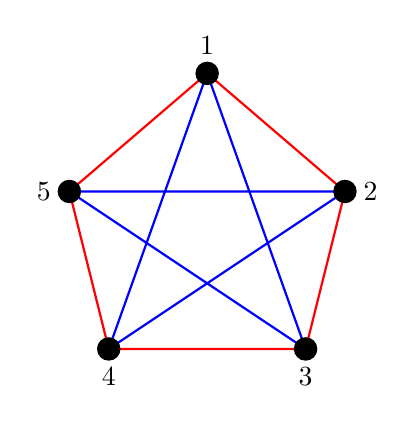
\begin{tikzpicture}[thick,scale=0.5]
        \coordinate (A) at (0,0);
        \coordinate (B) at (5,0);
        \coordinate (C) at (6,4);
        \coordinate (D) at (2.5,7);
        \coordinate (E) at (-1,4);
        \draw[red] (A) node[black, below, yshift=-3pt]{$4$}
        -- (B) node[black, below, yshift=-3pt]{$3$}
        -- (C) node[black, right, xshift=3pt]{$2$}
        -- (D) node[black, above, yshift=3pt]{$1$}
        -- (E) node[black, left, xshift=-3pt]{$5$}
        -- (A);
        \draw[blue] (A)--(D)--(B)--(E)--(C)--(A);
        \foreach \n in {A,B,C,D,E}
            \node at (\n)[circle,fill,inner sep=3pt]{};
    \end{tikzpicture}
\end{center}

请注意该图形优雅的对称性:所有红线均位于五边形的外侧,所有蓝线均位于该形状的内部。这样做的原因是,任意三个相邻点作为顶点的三角形必须使用两条外线和一条内线,任意三个不相邻点作为顶点的三角形必须使用两条内线和一条外线。(想一想:为什么我们不能用三条内线或三条外线来组成一个三角形?)这\emph{保证}了我们绘制的任何三角形都会使用两条不同颜色的线,所以这个图形不具有同质性!当然,我们可以查看图中所有可能的三角形,并确保它们都不使用一种颜色。这样的三角形有多少个?你能多快手工找到所有这些三角形?这样做是否更容易,或者注意我们上面提到的内部/外部属性?

也许你找到的解决方案与我们的图不同。你怎么知道它实际上是否是不同的图形?你的图中有多少条蓝线、多少条红线?我们的图呢?尝试通过移动点来重新绘制图形,但保持点之间的关系(即任意两个点之间绘制的线条的颜色)。你能把你的图形弄得跟我们的一样吗?你认为这对本题解的数量意味着什么?

\subsubsection*{$n=6$ 的情况}

好的,现在我们可以思考六个人的情况了。就点和线而言,我们希望用蓝色或红色线绘制六个点之间所有可能的连接,并确保不存在边都为相同颜色的三角形。在绘制前,请思考四个点和五个点时我们的解决方案。这些解是什么样的?这次我们要画多少线?我们可以试着让这个数字看起来像五个点的解决方案吗?有时,思考当前问题的解决方案与以前工作有何相似之处会大有帮助。现在,尝试画出这个图形,看看会发生什么。

有效吗?为什么无效?你在哪里遇到了麻烦?在不得不绘制单色三角形之前,你可以画多少条线?也就是说,在你绘制下一条线形成单色三角形之前,无论它是蓝色还是红色,你可以向图形中插入多少条线?某种程度上,这些问题对于解决这个特定难题来说是无关紧要的问题,但它们值得思考,因为它们本身很有趣,并且它们可能会引导我们找到这个难题的解决方案或其概括。为了便于说明,这是我们在图形中分配红线和蓝线的一种方案。我们为什么停在这里?还需要添加多少条线?我们能加进去吗?

\begin{center}
    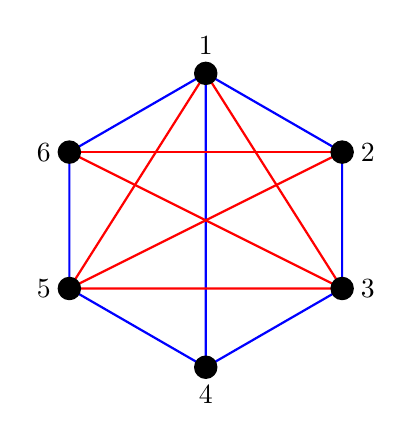
\begin{tikzpicture}[thick,scale=0.5]
        \coordinate (A) at (0,0);
        \coordinate (B) at (-3.4642,2);
        \coordinate (C) at (-3.4642,5.4642);
        \coordinate (D) at (0,7.4642);
        \coordinate (E) at (3.4642,5.4642);
        \coordinate (F) at (3.4642,2);
        \draw[blue] (A) node[black, below, yshift=-3pt]{$4$}
        -- (B) node[black, left, xshift=-3pt]{$5$}
        -- (C) node[black, left, xshift=-3pt]{$6$}
        -- (D) node[black, above, yshift=3pt]{$1$}
        -- (E) node[black, right, xshift=3pt]{$2$}
        -- (F) node[black, right, xshift=3pt]{$3$}
        -- (A)
        -- (D);
        \draw[red] (B)--(E);
        \draw[red] (C)--(F);
        \draw[red] (B)--(D)--(F)--(B);
        \draw[red] (C)--(E);
        \foreach \n in {A,B,C,D,E,F}
            \node at (\n)[circle,fill,inner sep=3pt]{};
    \end{tikzpicture}
\end{center}

我们现在面临的情况很有趣,因为它与我们之前面临的情况性质相反。在四个点和五个点的情况中,我们想表明\emph{可以}通过排列所有线来消除单色三角形。为了证明这一点,只需画出来就好!画出具有所需属性的\emph{特定}图形就足以证明可以实现我们想要的属性。然而,对于六个点,似乎不可能将线条排列得不存在单色三角形。我们怎样才能证明这是事实呢?我们很容易想到,只需考虑线条的所有可能排列,并论证每一中排列中至少有一个单色三角形。这可行吗?线条有多少种排列方式?我们如何在任意给定图形中轻松找到单色三角形?还记得我们对五个点的图形进行此操作吗?我们注意到,任何三角形都必须使用\emph{至少}一条来自外部的线和\emph{至少}一条来自内部的线,这保证了任何三角形都有两种类型的线。我们可以在这里做同样的事情,并明确一些\emph{保证}存在非单色三角形的性质吗?

问题是,图中六点之间线的可能排列方式太多了,我们无法手动完成所有检查!这里有 $15$ 条线需要绘制,每条线都可以是蓝色或红色,因此共有 $2^{15}$ 种可能的排列。这是一个很大的数字!(实际上,排列可能性会稍微少一些,因为其中一些排列在某种意义上是等价的;更专业地说,它们是``\emph{同构的}''。)

\subsubsection*{解答:处理\emph{任意}图形}

我们需要更巧妙地进行论证,这样我们就可以在不绘制特定图形的情况下证明\emph{任意}图形的性质。也就是说,我们需要找到一些事实,一些对所有可能的六点图都成立的性质,但我们仍然能够推断出一定存在三角形。解决这个问题的一种方法是考虑在图形的一小部分中绘制线条。具体来说,让我们取六个点中的任意一个,并考虑从该点引出的五条线。例如,我们可能会得到下面的图形:

\begin{center}
    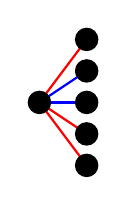
\begin{tikzpicture}[thick,scale=0.2]
        \coordinate (A) at (0,0);
        \coordinate (B) at (3,2);
        \coordinate (C) at (3,0);
        \coordinate (D) at (3,4);
        \coordinate (E) at (3,-2);
        \coordinate (F) at (3,-4);
        \draw[blue] (A)--(C);
        \draw[blue] (A)--(B);
        \draw[red] (A)--(D);
        \draw[red] (A)--(E);
        \draw[red] (A)--(F);
        \foreach \n in {A,B,C,D,E,F}
            \node at (\n)[circle,fill,inner sep=3pt]{};
    \end{tikzpicture}
\end{center}

有多少蓝线,多少红线?这在一定程度上是一个棘手的问题:我们并没有真正考虑任何\emph{特定}图形(如上面的图形),而是试图找到有关所有可能图形的事实。因此,我们不能太具体地回答这个问题。假设我们看到一个\textbf{任意}图形,我们必须提出一个无论该图形是什么都有效的论证。 

我们\emph{可以}这样说:必须至少有三条蓝线或三条红线。你明白为什么这是真的吗?使其不成立的唯一方法是从特定点出发,有两条(或更少)蓝线和两条(或更少)红线,共计四条(或更少)线。不过,我们必须画出所有可能的连接,因此应该有五条!(这个论证是``\emph{抽屉原理}''的一个例子。这个原理说的是,我们无法将两种不同颜色的五个物体放入两个不同盒子中,而不将三个同种颜色的物体放入一个盒子。对这类问题来说,抽屉原理是一个非常有用的策略,我们稍后将在 \ref{sec:section8.6} 节更详细地研究该原理。)

那么我们的立场是什么呢?我们从任意一个六个点、填满线的图形开始,到专注于一个特定的点;从这个点出来,一定有三条蓝线或三条红线。它可以是任意一种颜色,所以我们不能仅仅假设它是红色的并遵循这种假设进行论证;我们可以这样做,但之后必须回到这一点,看看如果这三条线是蓝色的,会发生什么变化。因此,让我们这样处理:让我们检查所有有三条红线从该特定点引出的图形。我们能得到什么?我们还没有对图中的其他线做出任何假设,所以让我们看看它们可能是什么。观察下图,看看到目前为止我们假设存在哪些线条颜色:

\begin{center}
    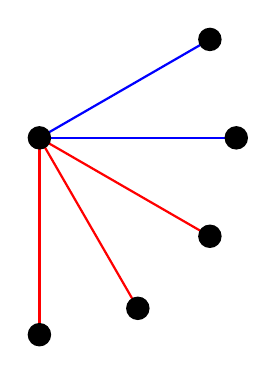
\begin{tikzpicture}[thick,scale=0.5]
        \coordinate (A) at (0,0);
        \coordinate (B) at (4.33,2.5);
        \coordinate (C) at (5,0);
        \coordinate (D) at (4.33,-2.5);
        \coordinate (E) at (2.5,-4.33);
        \coordinate (F) at (0,-5);
        \draw[blue] (A)--(C);
        \draw[blue] (A)--(B);
        \draw[red] (A)--(D);
        \draw[red] (A)--(E);
        \draw[red] (A)--(F);
        \foreach \n in {A,B,C,D,E,F}
            \node at (\n)[circle,fill,inner sep=3pt]{};
    \end{tikzpicture}
\end{center}

现在,可以在该图中添加哪些线而不会在三点之间形成同种颜色的三角形?我们不能对图中两个孤立点之间的线做任何假设,所以让我们关注底部的三个点。其中的线条可能是什么颜色?如果其中任何一条是红色的,那就会在该线的两个端点和我们关注的原始点之间形成一个单色三角形!这是有问题的。

\begin{center}
    \begin{tikzpicture}[thick,scale=0.5]
        \coordinate (A) at (0,0);
        \coordinate (B) at (4.33,2.5);
        \coordinate (C) at (5,0);
        \coordinate (D) at (4.33,-2.5);
        \coordinate (E) at (2.5,-4.33);
        \coordinate (F) at (0,-5);
        \draw[blue] (A)--(C);
        \draw[blue] (A)--(B);
        \draw[red] (A)--(D);
        \draw[red] (A)--(E);
        \draw[red] (A)--(F);
        \draw[red] (E)--(F);
        \draw [red,-stealth,very thick] (-2,-2.4) node[red, above]{$\text{红色三角形}$} -- (1,-3.5);
        \foreach \n in {A,B,C,D,E,F}
            \node at (\n)[circle,fill,inner sep=3pt]{};
    \end{tikzpicture}
\end{center}

避免这种情况的唯一方法是将所有这些线都变成蓝色。但这会在这三个点之间形成一个蓝色三角形!哇,看来无论我们做什么都无法避免生成单色三角形!

\begin{center}
    \begin{tikzpicture}[thick,scale=0.5]
        \coordinate (A) at (0,0);
        \coordinate (B) at (4.33,2.5);
        \coordinate (C) at (5,0);
        \coordinate (D) at (4.33,-2.5);
        \coordinate (E) at (2.5,-4.33);
        \coordinate (F) at (0,-5);
        \draw[blue] (A)--(C);
        \draw[blue] (A)--(B);
        \draw[red] (A)--(D);
        \draw[red] (A)--(E);
        \draw[red] (A)--(F);
        \draw[blue] (F)--(D)--(E)--(F);
        \draw [blue,-stealth,very thick] (5.5,-3.8) node[blue, right]{$\text{蓝色三角形}$} -- (2.5,-3.8);
        \foreach \n in {A,B,C,D,E,F}
            \node at (\n)[circle,fill,inner sep=3pt]{};
    \end{tikzpicture}
\end{center}

让我们回到抽屉原理并重新评估情况。如果原理保证的相同类型的三条线是蓝色而不是红色会怎样?其实,不会有什么改变。向图形底部的三个点之间添加新线,我们仍然会陷入困境:

\begin{center}
    \begin{tikzpicture}[thick,scale=0.5]
        {
            \coordinate (A) at (0,0);
            \coordinate (B) at (4.33,2.5);
            \coordinate (C) at (5,0);
            \coordinate (D) at (4.33,-2.5);
            \coordinate (E) at (2.5,-4.33);
            \coordinate (F) at (0,-5);
            \draw[red] (A)--(C);
            \draw[red] (A)--(B);
            \draw[blue] (A)--(D);
            \draw[blue] (A)--(E);
            \draw[blue] (A)--(F);
            \draw[blue] (E)--(F);
            \draw [blue,-stealth,very thick] (-2,-2.4) node[blue, above]{$\text{蓝色三角形}$} -- (1,-3.5);
            \foreach \n in {A,B,C,D,E,F}
                \node at (\n)[circle,fill,inner sep=3pt]{};
        }
        {
            \coordinate (A1) at (8,0);
            \coordinate (B1) at (12.33,2.5);
            \coordinate (C1) at (13,0);
            \coordinate (D1) at (12.33,-2.5);
            \coordinate (E1) at (10.5,-4.33);
            \coordinate (F1) at (8,-5);
            \draw[red] (A1)--(C1);
            \draw[red] (A1)--(B1);
            \draw[blue] (A1)--(D1);
            \draw[blue] (A1)--(E1);
            \draw[blue] (A1)--(F1);
            \draw[red] (F1)--(D1)--(E1)--(F1);
            \draw [red,-stealth,very thick] (13.5,-3.8) node[red, right]{$\text{红色三角形}$} -- (10.5,-3.8);
            \foreach \n in {A1,B1,C1,D1,E1,F1}
                \node at (\n)[circle,fill,inner sep=3pt]{};
        }
    \end{tikzpicture}
\end{center}

如果我们加入任何蓝色线,它就会与原始点形成一个单色三角形,如果我们将它们全部变成红色,就会在那三个点间形成一个单色三角形!从这个意义上讲,我们在抽屉原理之后遵循的两个论证是\emph{相同的}。如果我们用``红色''替换``蓝色''一词,反之亦然,我们会得到相同的论点。有时,数学家会利用这种情况来简化证明,只说``不失一般性,三条线是红色的''。这通常意味着,如果我们做出其他选择(即,如果线是蓝色的),那么进一步的论证在数学上将具有相同的结构,因此我们可以不重复书写相同的文字来节省时间和空间。事实上,这种情况非常常见,以至于有时你可能会看到``不失一般性''这个短语缩写为 \textbf{WOLOG} 或 \textbf{WLOG}。

\subsubsection*{解答:总结结果}

到目前为止我们取得了什么成果?我们绘制了\emph{特定}的图形,表明我们可以将线条排列在四个和五个点之间,而不出现单色三角形,并且我们认为\emph{任何}由六个点构成的图\emph{一定}具有单色三角形。就题目中朋友/敌人的表述而言,这意味着任何六人组必然存在一个三人组,其中的成员要么都是朋友要么都是敌人。

请注意,把这个问题改写成这个点/线的形式是多么有帮助;它让我们完全忘记了问题的社交背景(某种程度上,这可能会分散注意力),并简化了术语和符号(我们将成对的人标记为``朋友''或``敌人''变为简单地绘制两点之间一条线)。这是一个非常有用的策略:提取谜题的内在结构 --- 底层工作、元素之间的关系、它们如何相互作用等 --- 并根据这些部分重写所有内容。这可以使难题变得更容易理解和解决,并且可以指导我们设计更好的符号。如果我们继续用 $13F, 23E, \dots$ 这种符号来解决这个问题会怎样?也许最终能解决,但会困难得多!

这个题目最初的问题之一是确定一个下界,使得任何更大的人群都必然拥有该子群属性。你认为我们已经做到了吗?我们确定了一个下界了吗?六可能是这个数字吗?为什么是或为什么不是?在任意七人组中,都有一个较小的六人组,而我们上面的工作证明该小组中必然存在三个共同的朋友/敌人!当然,这适用于任何人数超过六人的群体,因此这一定是我们要寻找的精确下界。这与题目原始陈述中提到的结果类似,匈牙利社会学家在规模为四的子群中注意到了这种现象。这个问题解决起来要困难得多,所以我们这里解决了一个更小、更简单的案例。这两个结果都与称为\textbf{拉姆齐理论}的一大类问题有关。组合学和图论的这个分支致力于识别这些``下界'',随着某种结构(如一群人)的规模不断增长,最终会出现一个点,我们可以\emph{保证}找到一个具有某种属性的子群(三个共同的朋友/敌人)。起初被认为是一种社会学现象,后来被证明是严格的数学事实。牛不牛!

\subsubsection*{泛化:留给你的问题}

在继续之前,让我们提出一些有趣且相关的问题。如果我们要寻找不同规模的同质群(例如四个、五个或十二个)该怎么办?当然,总的来说,我们必须有更多的人才能保证找到这样的子群。我们可以一直这样做吗?也就是说,给定任何所需的子群大小,我们可以像上面那样确定一个下界吗?即使没有找到特定的数字,你能想出如何证明这样的下界一定存在吗?此外,如果我们允许第三种可能:朋友、敌人、陌生人,又会怎样呢?我们可以回答关于同质群的类似问题吗?这些都与拉姆齐理论相关,甚至其中一些问题相当难以回答,需要数学家多年努力才能解决。许多此类简单问题仍然是悬而未决的、未解难题!如果你在这些问题上没有任何进展,请不要灰心。我们相信,对这些问题的任何尝试和思考都是有意义且有益的。

\subsubsection*{解题心得}

这个问题带来了几个困难。首先,我们必须找到一种方法来以有意义的方式解释谜题,以便我们可以解决这个问题,这涉及到提出适当的符号来表示题目的元素。这是解决数学问题的重要组成部分,特别是这种不将符号和可视化作为问题陈述一部分的问题。

其次,为了确定 6 是群规模下界,我们必须以某种方式证明某些事情是\emph{不}可能的,但要检验的可能情况数量太大,无法单独检验每种情况。这种情况经常发生,特别是在与计算机科学和算法相关的问题中。为了解决这个问题,我们必须采用一种比大力出奇迹更巧妙的策略,而且并不总是清楚该采取什么策略。在这里,我们先是尝试填入线,就好像它会成功一样,然后意识到我们已经达到了一个无法添加的地步。证明某件事是可能的,相当于只是展示该现象的一个例子(我们对四人和五人组就是这么做的),但证明某件事是\emph{不可能}的可能要棘手得多,并且需要一些依赖上下文的独创性。

最后,我们发现,思考与当前问题密切相关的问题可能会很有趣,这些相关问题往往只需调整原问题的一个或多个条件。如果我们寻找更大的子群怎么办?如果我们允许更多类型的线怎么办?这将如何改变结果?通过改变这些条件来探索问题的边界可以带来新的数学发现和技术,并促使数学家积极探寻新的知识和分享知识的方法。

\clearpage


% !TeX root = ../../../book.tex
\subsection{三门问题}

\subsubsection*{问题描述}

这个问题仅涉及基础概率与算术,但多年来却让无数聪明人折戟沉沙。1990 年,玛丽莲·沃斯·萨万特 (Marilyn vos Savant) 在《Parade》杂志专栏发表该问题及其解法后,引发了激烈争论,许多人(包括数学家)致信赞同或反对她(正确)的答案。让我们看看你的见解!

\begin{quote}
    假设你正在参加一档游戏节目,面前有三扇门。其中一扇门后是汽车,其余两扇后是山羊。游戏开始前,汽车和山羊的位置已被随机放置在门后。游戏规则如下:你选定一扇门后,该门暂时保持关闭。主持人蒙蒂·霍尔 (Monty Hall) 知晓门后的情况,他会打开其余两扇门中有山羊的一扇。若两扇门后皆为山羊,他会随机开启一扇。蒙蒂·霍尔打开一扇有山羊的门后,会询问你:是坚持最初的选择,还是切换至另一扇关闭的门?试想:你选择了 1 号门,主持人打开了藏有山羊的 3 号门,然后问你:``是否要换到 2 号门?''改变最初的选择对你有利吗?
\end{quote}

当然,我们假设你更希望赢得汽车而非山羊,且力求最大化获胜概率。值得一提的是,该问题得名于电视节目《\emph{Let's Make a Deal}》的主持人蒙蒂·霍尔 (Monty Hall)。

那么你怎么想?试想自己站在聚光灯下,面对所有观众,当蒙蒂·霍尔问你:``要换到另一扇门吗?'' 你会作何选择?

请仔细思考一下,然后再翻页阅读解答。

\clearpage

\subsubsection*{结论:\emph{坚决}切换}

我们直接给出结论——该结论可能令人惊讶:你应当改变最初的选择!推理过程才是棘手且令人困惑的部分,而如何建立正确的解题思路正是该问题长期困扰求解者的原因。

\subsubsection*{错误论证分析}

首先展示一个常见的错误``解答'',该解答声称换门与否无关紧要。假设你与朋友讨论此题时对方提出如下解释,你会如何回应?该论证是否成立?若不同意,你会如何指出其谬误?

\begin{quote}
    当我选定一扇门后,蒙蒂·霍尔展示了另一扇有山羊的门,此时只剩两扇关闭的门。一扇后有山羊,另一扇后有汽车,因此我最初选择的门后有汽车的概率为 $50\%$,另一扇门后有汽车的概率也为 $50\%$。因此,换门不换门没有区别,还不如坚持最初的选择。
\end{quote}

上面的解释能说服你吗?让我们揭示其根本缺陷。解决此问题的关键在于计算两个概率值:坚持原选择获胜的概率,以及换门后获胜的概率。唯有准确计算并比较这两个值,才能彻底解决这个难题。

上述论证将两个概率均视为 $50\%$,但其推理存在根本缺陷。你认为坚持原选择获胜的真实概率是多少?关键在于:展示有山羊的门的行为并不会影响最初选择的门后的物体。请重点理解以下陈述:

\begin{quote}
    因为有三扇门,所以一开始选择正确的门的概率是 $\frac{1}{3}$,看到另一扇门后面有山羊\emph{并不能改变这一事实}。
\end{quote}
这正是上面错误论证的核心症结,也是``解答''本题时最常见的误区。

接下来计算换门后的胜率,并将其与 $\frac{1}{3}$ 进行比较。事实上,有多种方法可以计算此概率。一种简洁的推导是:只要初始选择的门后是山羊(概率 $\frac{2}{3}$),换门必然获胜(赢得汽车)。因为此时两扇未选门中藏着山羊与汽车,主持人必定展示有山羊的门,剩余那扇门后必定是汽车。因此换门策略的胜率为 $\frac{2}{3}$。

\subsubsection*{枚举可能性}

上述解释可能无法令你信服,我们不妨尝试实际枚举门后山羊与汽车的可能排列,并具体分析每种情况下切换选择的结果。首先请注意,门的编号并无实质影响,因为所有选择都是随机的;也就是说,无论汽车停在 1 号门、2 号门还是 3 号门后,我们最初选中汽车的概率始终是 $\frac{1}{3}$。因此可 \textbf{WOLOG}(此缩写意为``不失一般性'')假设汽车位于 1 号门后,山羊分别在 2 号门和 3 号门后。需要强调的是,这是我们自己设定的条件,参赛者并不知晓(否则必然直接选择 1 号门!)。基于此设定,我们考察初始选择的全部三种情况:

\begin{center}
    \begin{tabular}{ c|c|c } 
     1 号门 & 2 号门  & 3 号门 \\ 
     \hline 
     汽车   & 山羊    & 山羊 \\
    \end{tabular}
\end{center}

\begin{center}
    \begin{tabular}{ c|c|c|c } 
     我们的选择 & 主持人展示 & 换门结果 & 不换门结果 \\ 
     \hline 
     1 号门    & 2 号门 \:或\: 3 号门  & 山羊 & 汽车 \\
     2 号门    & 3 号门            & 汽车 & 山羊 \\
     3 号门    & 2 号门            & 汽车 & 山羊 \\
    \end{tabular}
\end{center}

关键发现在于:当我们初始选中有汽车的门时,主持人可以随机开启任意一扇有山羊的门。但无论开启哪扇门,切换选择都将失败,而坚持选择会获胜。这种情况仅占 $\frac{1}{3}$,即初始选中汽车的概率。由于表中所有情况概率均等,可以得出结论:切换策略的胜率为 $\frac{2}{3}$,而坚持策略的胜率仅为 $\frac{1}{3}$。

现在是否感觉问题更清晰了?不妨向亲友提出这个问题并观察他们的反应:有多少人答对?多少人能正确解释?多少人误答``概率相同''?又有多少人此前已经接触过此题?

\subsubsection*{泛化到多门多车情形}

让我们将这个游戏节目问题泛化,分析切换策略是否仍然有效。假设共有 $n$ 扇门和 $m$ 辆汽车,因此有 $n - m$ 只山羊。为进行有效分析,需满足 $m \le n - 2$,原因如下:

\begin{itemize}
    \item 如果 $m = n$,则无论切换与否都必然获胜,无需讨论。
    \item 如果 $m = n-1$,当初始选择有山羊的门时,主持人\emph{无法}展示另一扇有山羊的门,游戏规则无法成立,切换策略也就毫无意义。
\end{itemize}

现在,有了这些变量,游戏的新规则如下:我们随机选择一扇门。主持人从\emph{其余}门中随机打开一扇有山羊的门。此时可选择坚持最初选择或切换至\emph{任意}未打开的门。关键问题是:最优策略是什么?切换是否有利?答案是否取决于 $m$ 和 $n$?

我们将用与原题中第一种方法大致相同的方式来处理这道修改后的问题。由于 $m,n$ 为变量,我们无法枚举所有情况,只能采用逻辑推理来推断坚持和切换的胜率。首要观察与原始问题一致:\emph{坚持策略}的胜率等于初始选中汽车的概率。若初始选中有汽车的门(概率 $\frac{m}{n}$),坚持必胜;若选中有山羊的门(概率 $\frac{n-m}{n}$),坚持必败。故坚持策略的胜率为 $\frac{m}{n}$。

为了计算切换策略的胜率,需要分两种情况讨论。请注意,当 $m \geq 2$ 时,初始选中有汽车的门后切换仍可能获胜。考虑到这一点,我们需要分两种不同情况讨论:(a) 初始选中有山羊的门的情况,(b) 初始选中有汽车的门的情况。每种情况都会给主持人留下不同数量的选择,进而留下不同数量的切换策略和获胜方式,所以此处需要分开处理。

\begin{enumerate}[label=(\alph*)]
    \item \textbf{初始选中有山羊的门}。现在还剩下 $n - m - 1$ 扇有山羊的门,主持人随机选择其中一扇打开。从我们的角度来看,切换给我们留下了 $n-2$ 个选项(我们不能切换到已打开的门和最初选择的门),其中 $m$ 个是汽车。因此,在这种\emph{特定}情况下,切换后获胜的概率为 $\frac{m}{n-2}$。\\
    由于最初有 $n - m$ 只山羊,所以这种情况发生的概率为 $\frac{n-m}{n}$。因此,这种情况对切换后总获胜概率的贡献为
    \[\frac{n-m}{n} \cdot \frac{m}{n-2} = \frac{nm-m^2}{n(n-2)}\]
    (思考一下为什么我们要把这些概率相乘而不是相加?我们要如何将此概率与下一种情况的概率结合起来?)
    \item \textbf{初始选中有汽车的门}。现在还剩下 $n - m$ 扇有山羊的门,主持人随机选择其中一扇打开。从我们的角度来看,切换给我们留下了 $n-2$ 个选项,其中 $m - 1$ 个是汽车。因此,在这种\emph{特定}情况下,切换后获胜的概率为 $\frac{m-1}{n-2}$。\\
    由于最初有 $m$ 辆车,所以这种情况发生的概率为 $\frac{m}{n}$。因此,这种情况对切换后总获胜概率的贡献为
    \[\frac{m}{n} \cdot \frac{m-1}{n-2} = \frac{m^2-m}{n(n-2)}\]
\end{enumerate}

由于这两种情况是独立发生的(即它们不可能同时发生),我们需要将这两个概率相加,从而得到切换策略的总胜率:
\begin{align*}
    \frac{nm-m^2}{n(n-2)} + \frac{m^2-m}{n(n-2)} &= \frac{nm - m^2 + m^2 - m}{n(n-2)} \\
    &= \frac{nm - m}{n(n-2)} \\
    &= \frac{m(n - 1)}{n(n-2)} \\
    &= \frac{m}{n} \cdot \frac{n-1}{n-2}
\end{align*}
将此结果与坚持策略的胜率 $\frac{m}{n}$ 比较。因为 $ n - 1 > n - 2$,所以 $\frac{n-1}{n-2} > 1$,可得不等式:
\[\frac{m}{n} < \frac{m}{n} \cdot \underbrace{\frac{n-1}{n-2}}_{>1}\]
切换策略的胜率\emph{严格大于}(即总是大于)坚持策略的胜率。因此,随机切换到另一扇门总是更优策略!

\subsubsection*{具体应用}

此问题的原始版本对应 $n = 3$ 且 $m = 1$,因此可以将这些值代入来验证结果的正确性。根据推导公式,坚持策略的胜率为 $\frac{1}{3}$,而切换策略的胜率为 $\frac{1(3-1)}{3(1)} = \frac{2}{3}$,与之前的结论完全吻合!

\subsubsection*{泛化:留给你的问题}

当 $m$ 和 $n$ 取其他值时会发生什么?能否使``始终切换''策略显著优于``始终坚持''策略?两种策略的胜率差异最大能达到多少?最小又能缩小至何种程度?是否存在使两者胜率相等的情况?

该问题的另一变体是主持人开启多于一扇有山羊的门。具体设定如下:共有 $n$ 扇门,其中 $m$ 扇后有汽车;玩家首次选择后,主持人从剩余门中随机开启 $p$ 扇有山羊的门;此时玩家可选择坚持初始选择,或切换到未开启的 $n-p-1$ 扇门中的任意一扇。在此情形下最优策略是什么?需对 $m,n,p$ 施加何种约束条件以保证游戏成立?最优策略是始终切换,还是取决于 $p$ 的取值?``始终切换''与``始终坚持''策略的胜率差异范围如何?

\subsubsection*{解题心得}

直觉和快速决策有时能\emph{引导}我们找到正确答案,但务必检查这些仓促判断是否基于合理的逻辑。本题中,``$50/50$''的概率初看似乎成立,但仔细推敲后便发现其论证存在缺陷——关键在于正确解读题目并严格遵循游戏步骤的顺序。概率分析应按照游戏实际发生的流程进行,而非从结果倒推。

概率问题往往极具迷惑性,需格外审慎对待。这也揭示了一个深刻启示:看似简单的问题往往最难攻克。切勿因表述简短或易于理解而轻视问题的复杂性!

关于蒙蒂·霍尔问题及其心理学背景,请参见 \href{http://www.usd.edu/~xtwang/Papers/MontyHallPaper.pdf}{Krauss, Stefan and Wang, X. T. (2003). ``The Psychology of the Monty Hall Problem: Discovering Psychological Mechanisms for Solving a Tenacious Brain Teaser'', \emph{Journal of Experimental Psychology}: General 132(1)}。